\documentclass[letterpaper,11pt, reqno]{amsart}

\usepackage{amsfonts, amsthm, amssymb, amsmath, stmaryrd}
\usepackage{bbm}
\usepackage{mathrsfs,array}
\usepackage{eucal,fullpage,times,color,enumerate,accents,mathtools}
\usepackage{url}
\usepackage{scalerel,stackengine}
\usepackage{dotlessj}
\usepackage{cancel}
\usepackage{pgfplots}
\usepackage{colortbl,hhline}
\usepackage{tikz}
\usetikzlibrary{decorations.pathmorphing}
\usetikzlibrary{patterns}
\usetikzlibrary{arrows}
\usepackage[all]{xy}
\usepackage{soul}
\usepackage{xcolor}
\usepackage{etoolbox}
\usepackage{pifont}
\usetikzlibrary{fadings}
\usetikzlibrary{calc}
\usepackage{listings}
\usepackage{wasysym}
\tikzfading[name=fade out,
  inner color=transparent!0, outer color=transparent!100]
\tikzfading[name=fade right,
  left color=transparent!0, right color=transparent!100]
\tikzfading[name=fade left,
  right color=transparent!0, left color=transparent!100]
\tikzfading[name=fade mid,
  left color = transparent!100, right color = transparent!100, middle color=transparent!0]
\usepackage{ifthen}
\tikzset{
  laser beam action/.style={
    line width=\pgflinewidth+1.4pt,draw opacity=.095,draw=#1,
  },
  laser beam recurs/.code 2 args={%
    \pgfmathtruncatemacro{\level}{#1-1}%
    \ifthenelse{\equal{\level}{0}}%
    {\tikzset{preaction={laser beam action=#2}}}%
    {\tikzset{preaction={laser beam action=#2,laser beam recurs={\level}{#2}}}}
  },
  laser beam/.style={preaction={laser beam recurs={20}{#1}},draw opacity=1,draw=#1},
}
\usepackage{graphics}
\usepackage{graphicx}
\usepackage[export]{adjustbox}
\usepackage[curve]{xypic}
\usepackage{bm}
\usetikzlibrary{calc}
\usepackage[font=small,labelfont=bf]{caption}
\usepackage{stackengine,scalerel,graphicx}
\savestack\UAtextstyle{\stackon[-2.7pt]{$\rule[2.3pt]{4pt}{.35pt}$}{\scalebox{-1}{$U$}}}
\def\UA{\scalerel*{\UAtextstyle}{X}}
\usepackage{arydshln}



\definecolor{navy}{rgb}{0,0,.65}

%This reverse-links the references in the paper. Useful for large papers.
\usepackage[colorlinks]{hyperref}
\hypersetup{colorlinks=true,urlcolor=teal,linkcolor=navy,citecolor=navy}

\makeatletter
\def\@tocline#1#2#3#4#5#6#7{\relax
  \ifnum #1>\c@tocdepth % then omit
  \else
    \par \addpenalty\@secpenalty\addvspace{#2}%
    \begingroup \hyphenpenalty\@M
    \@ifempty{#4}{%
      \@tempdima\csname r@tocindent\number#1\endcsname\relax
    }{%
      \@tempdima#4\relax
    }%
    \parindent\z@ \leftskip#3\relax \advance\leftskip\@tempdima\relax
    \rightskip\@pnumwidth plus4em \parfillskip-\@pnumwidth
    #5\leavevmode\hskip-\@tempdima
      \ifcase #1
       \or\or \hskip 1em \or \hskip 2em \else \hskip 3em \fi%
      #6\nobreak\relax
    \dotfill\hbox to\@pnumwidth{\@tocpagenum{#7}}\par
    \nobreak
    \endgroup
  \fi}
\makeatother



\renewcommand{\familydefault}{ppl}
\setlength{\marginparwidth}{1in}
\setlength{\marginparsep}{0in}
\setlength{\marginparpush}{0.1in}
\setlength{\topmargin}{0in}
\setlength{\headheight}{0pt}
\setlength{\headsep}{0pt}
\setlength{\footskip}{.3in}
\setlength{\textheight}{9.0in}
\setlength{\textwidth}{6.25in}
\setlength{\parskip}{0pt}

%\newtheorem{theorem}{Theorem}[section]
\newtheorem{idea}{Musical proto-idea}[]
\renewcommand*{\theidea}{\arabic{idea}}
\newtheorem{ideaB}{Simple musical idea}[]
\renewcommand*{\theideaB}{\arabic{ideaB}}
\newtheorem{composition}{Composition}[]
\renewcommand*{\thecomposition}{\Alph{composition}}
\newtheorem{theorem}{Theorem}[subsection]
\newtheorem{monodromy theorem}{Monodromy Theorem}[subsection]
\newtheorem{corollary}[theorem]{Corollary}
\newtheorem{hypothesis}[theorem]{Hypothesis}
\newtheorem{wild conjecture}[theorem]{Wild Conjecture}
\newtheorem{claim}[theorem]{Claim}
\newtheorem{lemma}[theorem]{Lemma}
\newtheorem{proposition}[theorem]{Proposition}
\newtheorem{definition}[theorem]{Definition}
\newtheorem{warning}[theorem]{Warning}
\newtheorem{research objectives}{Research objectives}[subsection]
\newtheorem{questions}{Question}
\newtheorem{question}[theorem]{Question}
\newtheorem{research question}[theorem]{Research questions}
\newtheorem{answer}[theorem]{Answer}
\newtheorem{aside question}[theorem]{Aside question}
\newtheorem{exercise}[theorem]{Exercise}
\newtheorem{sketch}[theorem]{Sketch}
\newtheorem{aside}[theorem]{Aside}
\newtheorem{problem}[theorem]{Problem}
\newtheorem{conjecture}[theorem]{Conjecture}
\newtheorem{assumption}[theorem]{Assumption}
\newtheorem{construction}[theorem]{Construction}
\newtheorem{example}[theorem]{Example}
\newtheorem{examples}[theorem]{Examples}
\newtheorem{audio example}[theorem]{\loudspeaker[3] Example}
\newtheorem{quasi-theorem}[theorem]{Quasi-Theorem}
\newtheorem{prop/def}[theorem]{Proposition/Definition}
\newtheorem{blank remark}[theorem]{}
\newtheorem{ssubsection}[theorem]{}
\newtheorem{terminology and comment}[theorem]{Terminology and comment}
\newtheorem{fact}[theorem]{Fact}
\newtheorem{computation}[theorem]{Computation}
\newtheorem{observation}[theorem]{Observation}
\newtheorem{algorithm}[theorem]{Algorithm}
\newtheorem{setup}[theorem]{Setup}
\newtheorem{purity hypothesis}[theorem]{Purity hypothesis}
\newtheorem{corollary of the purity hypothesis}[theorem]{Corollary of the purity hypothesis}

%Theorem indexed with letters A, B, C, ...
\newtheorem{Th}{Theorem}[]
\renewcommand*{\theTh}{\Alph{Th}}

\newtheorem{rem1}[theorem]{Remark}
\newenvironment{remark}{\begin{rem1}\em}{\end{rem1}}

\newtheorem{not1}[theorem]{Notation}
\newenvironment{notation}{\begin{not1}\em}{\end{not1}}

%% Math Blackboard
\newcommand{\A}{{\mathbb{A}}}           
\newcommand{\CC} {{\mathbb C}}       
\newcommand{\DD} {{\mathbb D}}
\newcommand{\EE}{\mathbb{E}}
\newcommand{\GG}{\mathbb{G}}
\newcommand{\LL}{\mathbb{L}}
\newcommand{\NN} {{\mathbb N}}		
\newcommand{\PP}{\mathbb{P}}         
\newcommand{\QQ} {{\mathbb Q}}		
\newcommand{\RR} {{\mathbb R}}		
\newcommand{\Circ} {{\mathbb S}}		
\newcommand{\ZZ} {{\mathbb Z}}		
\newcommand{\TT} {{\mathbb T}}	
\newcommand{\FF}{{\mathbb F}}

%%Presuperscript
\def\presuper#1#2%
  {\mathop{}%
   \mathopen{\vphantom{#2}}^{#1}%
   \kern-\scriptspace%
   #2}
	
\newcommand{\BC}{\text{BC}}

\DeclareMathOperator{\Aut}{Aut}
\DeclareMathOperator{\Gal}{Gal}
\DeclareMathOperator{\Circpec}{Spec_{\ \!}}
\DeclareMathOperator{\Split}{split}
\DeclareMathOperator{\Div}{div}
\DeclareMathOperator{\ord}{ord_{\ \!}}

\newcommand{\model}[1]{{\slantbox[.5]{$\mathcal{#1}$}\ }}

\newcommand{\lra}{{\longrightarrow}}
\DeclareMathOperator{\Def}{\overset{{}_{\text{def}}}{=}}

% slant box
\newsavebox{\foobox}
\newcommand{\slantbox}[2][.5]
  {%
    \mbox
      {%
        \sbox{\foobox}{#2}%
        \hskip\wd\foobox
        \pdfsave
        \pdfsetmatrix{1 0 #1 1}%
        \llap{\usebox{\foobox}}%
        \pdfrestore
      }%
  }

%%Prettier monomorphism and epimorphism arrows
\newcommand{\mono}{\!\xymatrix{{}\ar@{^{(}->}[r]&{}}\!}
\newcommand{\epi}{\!\xymatrix{{}\ar@{->>}[r]&{}}\!}
\newcommand{\rat}{\!\xymatrix{{}\ar@{-->}[r]&{}}\!}

%%Young diagram
\newcommand{\young}{\scalebox{.7}{$\pmb{\square\!\square}${\larger\larger $\pmb{\cdot\!\cdot\!\cdot}$}$\pmb{\square}$}}

%smaller subscript closed field
\newcommand{\lilF}{\mbox{{\smaller\smaller\smaller\smaller\smaller $\overline{\FF_{\!q}}$}}}

\newcommand{\iso}{\cong}
\newcommand{\disc}{\text{disc}}

% Tyler comments
\newcommand{\tyler}[1]{{\color{red} [#1\ \ \textemdash Tyler]}}

% Some slanted letters
\newcommand{\TP}{\slantbox[.3]{$\mathcal{TP}$}}

%Left action
\newcommand{\lact}{\ \raisebox{8pt}{\rotatebox{-90}{$\circlearrowright$}}\ }

%Left quotient
\newcommand{\lquot}[2]{\raisebox{-1.5pt}{$#1$}\big\backslash\raisebox{1.5pt}{$#2$}}

%Right quotient
\newcommand{\rquot}[2]{\raisebox{1.5pt}{$#1$}/\raisebox{-1.5pt}{$#2$}}

%importantmatrix
\newcommand{\MM}{\big(\begin{smallmatrix}0 & -1\\ 1 & -1\end{smallmatrix}\big)}

%compactified spec
\newcommand{\SpecZN}[1]{\overline{\text{Spec}_{\ \!}\ZZ}{}^{(#1)}}
\newcommand{\SpecZ}{\overline{\text{Spec}_{\ \!}\ZZ}}

%nice sep
\newcommand{\sep}{\textsf{sep}}

%nice res
\newcommand{\res}{\text{res}^{\eta}_{s}}

%nice sp
\newcommand{\spe}{\bold{Sp}}

%nice Sh
\newcommand{\Sh}{\bold{Sh}}

%nice et
\newcommand{\et}{\text{\'et}}

%nice M_g bar
\newcommand{\Mg}{{\ \ \overline{\!\!\mathscr{M}_{g}}}}
\newcommand{\Mgmbar}{\overline{M_{g}{\!\!}^{\text{{\smaller\smaller\smaller\smaller\smaller $\ (m)$}}}}}
\newcommand{\Mgm}{M_{g}{\!\!}^{\text{{\smaller\smaller\smaller\smaller\smaller $\ (m)$}}}}




%changed footnote style
\renewcommand{\thefootnote}{[\arabic{footnote}]}

\numberwithin{equation}{theorem}

%
\newcounter{totfigures}

\providecommand\totfig{} 

\makeatletter
\AtEndDocument{%
  \addtocounter{totfigures}{\value{figure}}%
  \immediate\write\@mainaux{%
    \string\gdef\string\totfig{\number\value{totfigures}}%
  }%
}
\makeatother

\pretocmd{\chapter}{\addtocounter{totfigures}{\value{figure}}\setcounter{figure}{0}}{}{}


\newcommand{\midarrow}{\tikz \draw[-triangle 90] (0,0) -- +(.1,0);}



\usepackage{epigraph}
\setlength\epigraphwidth{.8\textwidth}
\setlength\epigraphrule{0pt}




\definecolor{codegreen}{rgb}{0,0.6,0}
\definecolor{codegray}{rgb}{0.5,0.5,0.5}
\definecolor{codepurple}{rgb}{0.58,0,0.82}
\definecolor{backcolour}{rgb}{0.95,0.95,0.92}

\lstdefinestyle{mystyle}{
    backgroundcolor=\color{backcolour},   
    commentstyle=\color{codegreen},
    keywordstyle=\color{magenta},
    numberstyle=\tiny\color{codegray},
    stringstyle=\color{codepurple},
    basicstyle=\ttfamily\footnotesize,
    breakatwhitespace=false,         
    breaklines=true,                 
    captionpos=b,                    
    keepspaces=true,                 
    numbers=left,                    
    numbersep=5pt,                  
    showspaces=false,                
    showstringspaces=false,
    showtabs=false,                  
    tabsize=2
}

\lstset{style=mystyle}





\newcommand{\ExternalLink}{%
    \tikz[x=1.2ex, y=1.2ex, baseline=-0.05ex]{% 
        \begin{scope}[x=1ex, y=1ex]
            \clip (-0.1,-0.1) 
                --++ (-0, 1.2) 
                --++ (0.6, 0) 
                --++ (0, -0.6) 
                --++ (0.6, 0) 
                --++ (0, -1);
            \path[draw, 
                line width = 0.5, 
                rounded corners=0.5] 
                (0,0) rectangle (1,1);
        \end{scope}
        \path[draw, line width = 0.5] (0.5, 0.5) 
            -- (1, 1);
        \path[draw, line width = 0.5] (0.6, 1) 
            -- (1, 1) -- (1, 0.6);
        }
    }


\usepackage{caption}
\captionsetup{font=footnotesize}

\usepackage{graphicx}
\newcommand\vcent[1]{\vcenter{\hbox{#1}}}
\newcommand\loudspeaker[1][3]{\ensuremath{\vcent{\rule{.6ex}{.6ex}}\kern-.5ex%
  \vcent{\scalebox{.6}[1]{\rotatebox[origin=center]{90}{$\blacktriangle$}}}%
  \ifnum#1>0\relax\kern.1ex\vcent{\scalebox{.4}{)}}\ifnum#1>1\relax\kern-.1ex%
  \vcent{\scalebox{.55}{)}}\ifnum#1>2\relax\kern-.15ex\vcent{\scalebox{.7}{)}}%
  \fi\fi\fi}%
}



\newcommand\modulo[2]{\@tempcnta=#1
        \divide\@tempcnta by #2
        \multiply\@tempcnta by #2
        \multiply\@tempcnta by -1
        \advance\@tempcnta by #1\relax
        \the\@tempcnta}
\makeatother


\makeatletter
\newcommand*{\doublerightarrow}[2]{\mathrel{
  \settowidth{\@tempdima}{$\scriptstyle#1$}
  \settowidth{\@tempdimb}{$\scriptstyle#2$}
  \ifdim\@tempdimb>\@tempdima \@tempdima=\@tempdimb\fi
  \mathop{\vcenter{
    \offinterlineskip\ialign{\hbox to\dimexpr\@tempdima+1em{##}\cr
    \rightarrowfill\cr\noalign{\kern.5ex}
    \rightarrowfill\cr}}}\limits^{\!#1}_{\!#2}}}
\newcommand*{\triplerightarrow}[1]{\mathrel{
  \settowidth{\@tempdima}{$\scriptstyle#1$}
  \mathop{\vcenter{
    \offinterlineskip\ialign{\hbox to\dimexpr\@tempdima+1em{##}\cr
    \rightarrowfill\cr\noalign{\kern.5ex}
    \rightarrowfill\cr\noalign{\kern.5ex}
    \rightarrowfill\cr}}}\limits^{\!#1}}}
\makeatother


\makeatletter
\def\@tempa#1{\@xp\@tempb\meaning#1\@nil#1}
\def\@tempb#1>#2#3 #4\@nil#5{%
  \@xp\ifx\csname#3\endcsname\mathaccent
    \@tempc#4?"7777\@nil#5%
  \else
    \PackageWarningNoLine{amsmath}{%
      Unable to redefine math accent \string#5}%
  \fi
}
\def\@tempc#1"#2#3#4#5#6\@nil#7{%
  \chardef\@tempd="#3\relax\set@mathaccent\@tempd{#7}{#2}{#4#5}}


\@tempa\widehat
\makeatother


%%%%%%%%%%%%%%%%%%%%%%%%%%%%%%%%%%%%%%
%%%%%%%%%%%%%%%%%%%%%%%%%%%%%%%%%%%%%%

\setcounter{tocdepth}{2}


\title{{\smaller\smaller\smaller\smaller\it Notes on}\\ \ \\ Tonal Theories\\ {\smaller\smaller\smaller\it coming from} Representations of\\ Algebraic Groups {\smaller\smaller\smaller\it other than} $\text{GL}_{\pmb{1}}\pmb{(\CC)}$\\ \ \\ \ {\smaller\smaller\smaller\smaller\it \textemdash\ In progess\ \textemdash}}
\date{\today}
\author{Tyler Foster}

\begin{document}

\maketitle

\begin{abstract}
   Lots of the structure of tonal harmony emerges from the representation theory of $\text{GL}_{1}(\CC)$. I here begin the project of composing music using tonal structures that emerge from the representation theory of other, higher-dimensional algebraic groups, such as $\text{SL}_{2}(\CC)$. This isn't just some theoretical exercise. As these notes should make clear, implementing these tonal structures in code will be very difficult to pull off without the super detailed outline of the general theory that appears below.
\end{abstract}

\tableofcontents

\begin{section}{Navigating tonality through the representation theory of $\text{GL}_{1}(\CC)$.}

\begin{subsection}{Sources}
	\begin{enumerate}[{\bf\ \ \ \ \ \ 1.}]
	\item
	\cite{Pont}
	\item
	\cite{Tao}
	\item
	\cite{TenneyScratch}
	\item
	\cite{Cohn}
	\item
	\cite{TenneyV1}
	\item
	\cite{NeoRie}
	\item
	\cite{Geo}
	\end{enumerate}
\end{subsection}

\begin{subsection}{Representation theory of $\text{GL}_{1}(\CC)$.} The {\em general linear group on the $1$-dimensional complex vector space $\CC$}, denoted $\text{GL}_{1}(\CC)$, is the group of invertible $1\times 1$-matrices under the operation of matrix multiplication. We have a natural identification with the multiplicative group of nonzero elements in $\CC$:
	$$
	\text{GL}_{1}(\CC)
	\ \cong\ 
	\CC^\times.
	$$
This multiplicative Abelian group $\CC^\times$ has a natural decomposition into the Cartesian product of the additive group $\text{log}(\RR^\times)$ and the circle group $\mathbb{S}^{1}$:
	$$
	\CC^\times\ \cong\ \text{log}(\RR^\times)\times\mathbb{S}^{1}.
	$$
This decomposition of $\CC^\times$ corresponds to the unique representation of any nonzero complex number $q$ as a product
	$$
	q
	\ =\ 
	e^{\text{log}(A)+i\omega},
	\ \ \ \ \ \ \text{with}\ \ \ 
	\text{log}(A)\in\RR
	\ \ \ \text{and}\ \ \ 
	0\le \omega<2\pi.
	$$
Here $A$ has units of $A_0 \ e^{20\ \text{dB}}$, where $A_{0}$ is some fixed reference amplitude. Thus $\text{log}(A)$ has units of $\text{log}(A_0)+20\ \text{dB}$, where $\text{log}(A_{0})$ is some fixed reference log-amplitude.\footnote{\ It's interesting how I can tell the ``what this has to do with music'' part of the story by naming units.} This $q$ has real and imaginary parts
	\begin{equation}\label{equation: connection to oscillators}
	\text{Re}\ q
	\ =\ 
	A\ \text{cos}(\omega)
	\ \ \ \ \ \ \text{and}\ \ \ \ \ \ 
	\text{Im}\ q
	\ =\ 
	A\ \text{sin}(\omega),
	\end{equation}
respectively. The functions of $\omega$ in Equation \eqref{equation: connection to oscillators} are what are sometimes, in music production, called pure oscillators. The latter oscillator is the $\frac{\pi}{4}$-phase shift of the former. In these notes, it will often often be useful to reason using the notation ``$e^{\text{log}(A)+i\omega}$,'' instead of the notation in Equation \eqref{equation: connection to oscillators}. This is because the notation ``$e^{\text{log}(A)+i\omega}$'' is more closely related to the theory of representations of algebraic groups, and becomes extremely useful when we move on to algebraic groups other than $\text{GL}_{1}(\CC)$. I think it is fair to think of $e^{\text{log}(A)+i\omega}$ as being an especially simple, highly formalized instance of a {\em klang}, with properties that make it work well as a primitive building block of complex kangs. One of the main things we will do in these notes is play with ideas about how klangs can move by playing with ways klangs can be built.

A somewhat hidden, made-up premise in these notes is that tonality reflects constraints on performance that makes the parameters of (1) {\em phase} and (2) {\em relative amplitude} random variables that sweep out natural cosets. Thus we restrict attention to the quotient group at right in the short exact sequence
	$$
	0
	\ \lra\ 
	\text{log}(\RR^\times)\xrightarrow{\ \ e^{(-)}\ }
	\text{GL}_{1}(\CC)
	\lra
	\mathbb{S}^{1}
	\lra
	1.
	$$

{\color{red} [Say something about how one would get back to $\bold{Rep}\big(\text{GL}_{1}(\CC)\big)$ through induction/restriction...]}

	We focus on the category $\bold{Rep}(\mathbb{S}^{1})$. {\color{red} [Decomposition above gives us a direct connection to music. Moving up along tensor powers (multiple interpretations) couple with octave equivalence in human perception corresponds directly to perfect fifths, major thirds, etc...]}
\end{subsection}

\begin{subsection}{Connection to Fourier series}
\ 	
\begin{subsubsection}
\normalfont
{\bf Timbre as some kind of high frequency tonality.}
\end{subsubsection}

\begin{subsubsection}
\normalfont
{\bf Rhythm as some kind of low frequency tonality.}
\end{subsubsection}

\ {\color{red} [...]}
\end{subsection}

\begin{subsection}{Tonnetze and movement through $\bold{Rep}(\mathbb{S}^{1})$.}
\ {\color{red} [...]}
\end{subsection}

\begin{subsection}{Modal changes and functors along homomorphisms $\mathbb{S}^{1}\longrightarrow\mathbb{S}^{1}$.}
\ {\color{red} [...]}

\begin{subsubsection}
\normalfont
{\bf Approximating functors and 12-TET.}
A
\end{subsubsection}

\begin{subsection}{Isomorphisms $(\RR\!\times\!\mathbb{S}^{1})^\wedge\cong\RR^\wedge\!\times\!\ZZ$ and $(\RR\!\times\!\pmb{\mu}_{n})^\wedge\cong\RR^\wedge\!\times\!\ZZ/n\ZZ$.}
\ {\color{red} [...]}

\end{subsection}

\end{subsection}

\end{section}

\vskip 1cm

\begin{section}{Representations of the $p$-adic groups $\mathbb{A}^{\!1}(\mathbb{Q}_{p})$ and $\text{GL}_{1}(\mathbb{Q}_{p})$.}



\begin{subsection}{Sources}
	\begin{enumerate}[{\bf\ \ \ \ \ \ 1.}]
	\item
	\cite[Chp. 4]{Guillot}\ \textemdash\ My favorite introductory text on $p$-adic fields and their extensions.
	\item
	\cite[Chp. XV: {\em J. T. Tate's thesis}, 1950]{CF}
	\item
	\cite[\S VII]{Lang}
	\end{enumerate}
\end{subsection}

\begin{subsection}{Adele-ish products}
\ 
{\color{red} [...]}

	$$
	\ZZ/p^{n_1}_{1}\ZZ
	\ \times\ 
	\ZZ/p^{n_2}_{2}\ZZ
	\ \times\ 
	\cdots
	\ \times\ 
	\ZZ/p^{n_{k}}_{k}\ZZ
	$$
For example
	$$
	\ZZ/2^{d}\ZZ
	\ \times\ 
	\ZZ/3^{e}\ZZ
	\ \times\ 
	\ZZ/5^{f}\ZZ,
	\ \ \ \text{such that}\ \ \frac{2^{d}3^{e}5^{f}}{P}
	\ \approx\!
	\underset{
	{\smaller\smaller\smaller\smaller
	\begin{array}{c}
	\text{20\ kHz, doubled for}
	\\
	\text{Nyquist–Shannon}
	\\
	\text{sampling theorem}
	\end{array}
	}\!\!
	}{\underbrace{40\ 000\ \text{Hz}}}.
	$$
The values $d=0$, $e=4$, $f=4$ achieve this. Moreover, since $2\in(\ZZ/3^{e}\ZZ)^{\times}$ and $2\in(\ZZ/5^{f}\ZZ)^{\times}$ for any $e,f\ge 1$, we have a natural octave equivalence in $\ZZ/3^e\ZZ\times\ZZ/5^f\ZZ$, giving us the multiplicative monoid
	$$
	\big(\ZZ/3^e\ZZ\times\ZZ/5^f\ZZ\big)\Big/2^{\ZZ}
	$$
controlling pitch-class movement. Observe that we have a surjective map
	$$
	\text{pr}_{e,f}:(\QQ_{3}\times\QQ_5)\big/2^{\ZZ}
	\epi
	\big(\ZZ/3^e\ZZ\times\ZZ/5^f\ZZ\big)\Big/2^{\ZZ}.
	$$
We will sometimes argue directly in $(\QQ_{3}\times\QQ_5)\big/2^{\ZZ}$, and then use the projection $\text{pr}_{e,f}$ to derive the appropriate computable approximation.

{\color{red} [...]}

\end{subsection}

\begin{subsection}{Characters and Fourier transforms over the additive {\em p}-adic group.}
We define a map
	\begin{equation}\label{equation: base character}
	\lambda_{1}:\mathbb{A}^{\!1}(\QQ_p)\lra\RR/\ZZ\cong\mathbb{S}^{1}
	\end{equation}
as follows. Given $a\in\QQ_p$, write
	$$
	a
	\ \ =\ \ 
	\underset{a_{-}}{
	\underbrace{a_{-n}\tfrac{1}{p^n}+a_{-n+1}\tfrac{1}{p^{n-1}}+\cdots+a_{-1}\tfrac{1}{p}}}
	+
	\underset{a_{+}}{
	\underbrace{
	a_0+a_1 p+a_2 p^2+\cdots
	}}.
	$$
Since $p^{n}a_{-}\in\ZZ$, we have $a_{-}\in\ZZ\big[\tfrac{1}{p}\big]$, and we can define
	$$
	\lambda_{1}(a)
	\ :=\ 
	\text{class of}\ a_{-}\ \text{in the quotient}\ \ZZ\big[\tfrac{1}{p}\big]\big/\ZZ.
	$$
Composing this with the embeddings
	$$
	\ZZ\big[\tfrac{1}{p}\big]\big/\ZZ
	\mono
	\QQ/\ZZ
	\mono
	\RR/\ZZ,
	$$
and we obtain a map as in Equation \eqref{equation: base character}. One checks that $\lambda_1$ is a homomorphism of Abelian groups, that
	$$
	\lambda_{1}(a+b)
	\ =\ 
	\lambda_{1}(a)+\lambda_{1}(b)
	\ \ \ \ \ \ \text{and}\ \ \ \ \ \ 
	\lambda_{1}(0)
	\ =\ 
	0.
	$$

	For each element $b\in\QQ_{p}$, we obtain a new homomorphism
	$$
	\lambda_{b}:\mathbb{A}^{\!1}(\QQ_{p})\lra\RR/\ZZ
	$$
defined by
	$$
	\lambda_{b}(a)\ :=\ \lambda_{1}(ba).
	$$
In this way, we obtain a bilinear pairing
	$$
	\lambda_{(-)}(-):
	\QQ_{p}\otimes_{\ZZ}\QQ_{p}\lra\RR/\ZZ.
	$$
One can show that this pairing is non-degenerate. In this way, we obtain an isomorphism between $\mathbb{A}^{\!1}(\QQ_{p})$ and its own Pontryagin dual. This is sometimes written
	$$
	\begin{array}{c}
	\lambda_{(-)}:\QQ^{+}_{p}\xrightarrow{\ \ \sim\ \ }\ \!\widehat{\QQ^{+}_{p}},
	\\[6pt]
	\ \ \ \ \ \ \ \ \ \ b\xmapsto{\ \ \ \ \ \ \ \ \ } \lambda_{b}.
	\end{array}
	$$
	
	This means that for each $b\in\QQ_{p}$, we obtain a distinct $\CC^\times$-valued character
	$$
	\chi_{b}:\mathbb{A}^{\!1}(\QQ_{p})\lra\CC^\times
	$$
defined by
	$$
	\chi_{b}(a)
	\ :=\ 
	e^{i2\pi\lambda_{b}(a)}.
	$$
These functions $\chi_{b}(-)$ play the role of ``pure oscillators'' in the Fourier analysis of complex-valued signals
	$$
	f:\QQ_{p}\lra\CC,
	$$
and the additive topological group $\QQ_{p}$ serves as the spectrum parametrizing the frequencies of these oscillators, with
	$$
	\chi_{b}(t)
	\ =\ 
	\chi_{1}(bt).
	$$
We define the Haar measure $da$ on $\QQ_{p}$ to be the unique translation invariant measure for which
	$$
	\int_{\ZZ_{p}}\!\!\!\!da\ =\ 1.
	$$
One important feature of this particular Haar measure is that it satisfies $d(ba)=|b|_{p}\ da$. Integrating against the characters $\chi_{b}$ with respect to this measure defines our Fourier transform in this setting:
	$$
	\widehat{f}(b)
	\ :=\ 
	\int_{\QQ_{p}}\!\!\!f(a)\ \chi_{b}(a)\ da.
	$$
Writing this out explicitly, we get a formula strikingly similar to the standard Fourier transform between signals on $\mathbb{S}^{1}$ and signals on $\ZZ\cong\widehat{\mathbb{S}^{1}}$:
	$$
	\widehat{f}(b)
	\ =\ 
	\int_{\QQ_{p}}\!\!\!f(a)\ e^{i2\pi\lambda_{1}(ba)}\ da.
	$$
In the present case, the double-dual introduces a change of sign in the argument:
	$$
	\widehat{\text{$\!\!\widehat{f}$}}
	(a)
	\ \ =\ \ 
	f(-a).
	$$

\ 
{\color{red} [...]}

\end{subsection}

\begin{subsection}{Computing Fourier transforms over $\mathbb{A}^{\!1}(\QQ_{p})$}
\ 
{\color{red} [Characterization of maps $f:\QQ_{p}\lra\CC$...]}

\ 
{\color{red} [A tutorial with examples...]}
\end{subsection}

\begin{subsection}{A class of tonnetze for $\mathbb{A}^{\!1}(\QQ_{p})$}
\ 
{\color{red} [...]}
\end{subsection}

\begin{subsection}{One approach to {\em p}-adic signals.}
It is well known that $\QQ_2$ is homeomorphic to the standard ``middle thirds'' Cantor set inside the real interval $[0,1]$, and that $\QQ_p$ is homeomorphic to an ``alternating $(2n-1)^\text{ths}$'' Cantor-like set inside the real interval $[0,1]$.
	\begin{figure}[ht]
	$$
	{\color{red} [...]}
	$$
	\caption{{\bf Cantor-like, ``alternating $\pmb{5^\text{ths}}$'' realization of $\pmb{\QQ_p}$.} {\color{red} [...]}} 
	\end{figure}

{\color{red} [...]}
	\begin{figure}[ht]
	$$
	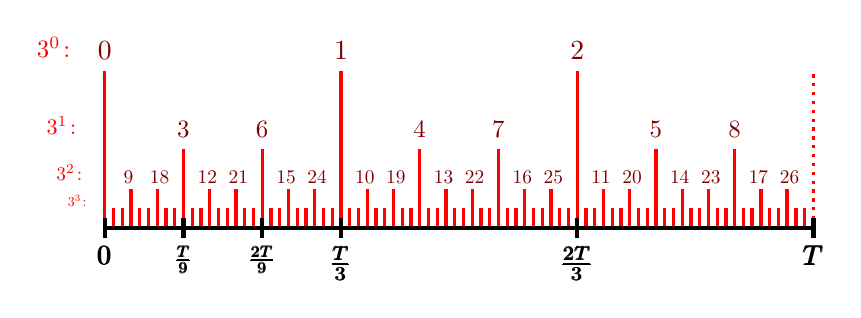
\begin{tikzpicture}
	\draw[red, very thick] (0,0) -- (0,2);
	\draw[red, very thick] (3,0) -- (3,2);
	\draw[red, very thick] (6,0) -- (6,2);
	\draw[red, very thick, dotted] (9,0) -- (9,2);
	%
	\draw[red, very thick] (1,0) -- (1,1);
	\draw[red, very thick] (2,0) -- (2,1);
	\draw[red, very thick] (4,0) -- (4,1);
	\draw[red, very thick] (5,0) -- (5,1);
	\draw[red, very thick] (7,0) -- (7,1);
	\draw[red, very thick] (8,0) -- (8,1);
	%
	\draw[red, very thick] (1/3,0) -- (1/3,.5);
	\draw[red, very thick] (2/3,0) -- (2/3,.5);
	\draw[red, very thick] (1+1/3,0) -- (1+1/3,.5);
	\draw[red, very thick] (1+2/3,0) -- (1+2/3,.5);
	\draw[red, very thick] (2+1/3,0) -- (2+1/3,.5);
	\draw[red, very thick] (2+2/3,0) -- (2+2/3,.5);
	\draw[red, very thick] (3+1/3,0) -- (3+1/3,.5);
	\draw[red, very thick] (3+2/3,0) -- (3+2/3,.5);
	\draw[red, very thick] (4+1/3,0) -- (4+1/3,.5);
	\draw[red, very thick] (4+2/3,0) -- (4+2/3,.5);
	\draw[red, very thick] (5+1/3,0) -- (5+1/3,.5);
	\draw[red, very thick] (5+2/3,0) -- (5+2/3,.5);
	\draw[red, very thick] (6+1/3,0) -- (6+1/3,.5);
	\draw[red, very thick] (6+2/3,0) -- (6+2/3,.5);
	\draw[red, very thick] (7+1/3,0) -- (7+1/3,.5);
	\draw[red, very thick] (7+2/3,0) -- (7+2/3,.5);
	\draw[red, very thick] (8+1/3,0) -- (8+1/3,.5);
	\draw[red, very thick] (8+2/3,0) -- (8+2/3,.5);
	%
	\draw[red, very thick] (1/9,0) -- (1/9,.25);
	\draw[red, very thick] (2/9,0) -- (2/9,.25);
	\draw[red, very thick] (1/3+1/9,0) -- (1/3+1/9,.25);
	\draw[red, very thick] (1/3+2/9,0) -- (1/3+2/9,.25);
	\draw[red, very thick] (2/3+1/9,0) -- (2/3+1/9,.25);
	\draw[red, very thick] (2/3+2/9,0) -- (2/3+2/9,.25);
	\draw[red, very thick] (3/3+1/9,0) -- (3/3+1/9,.25);
	\draw[red, very thick] (3/3+2/9,0) -- (3/3+2/9,.25);
	\draw[red, very thick] (4/3+1/9,0) -- (4/3+1/9,.25);
	\draw[red, very thick] (4/3+2/9,0) -- (4/3+2/9,.25);
	\draw[red, very thick] (5/3+1/9,0) -- (5/3+1/9,.25);
	\draw[red, very thick] (5/3+2/9,0) -- (5/3+2/9,.25);
	\draw[red, very thick] (6/3+1/9,0) -- (6/3+1/9,.25);
	\draw[red, very thick] (6/3+2/9,0) -- (6/3+2/9,.25);
	\draw[red, very thick] (7/3+1/9,0) -- (7/3+1/9,.25);
	\draw[red, very thick] (7/3+2/9,0) -- (7/3+2/9,.25);
	\draw[red, very thick] (8/3+1/9,0) -- (8/3+1/9,.25);
	\draw[red, very thick] (8/3+2/9,0) -- (8/3+2/9,.25);
	\draw[red, very thick] (9/3+1/9,0) -- (9/3+1/9,.25);
	\draw[red, very thick] (9/3+2/9,0) -- (9/3+2/9,.25);
	\draw[red, very thick] (10/3+1/9,0) -- (10/3+1/9,.25);
	\draw[red, very thick] (10/3+2/9,0) -- (10/3+2/9,.25);
	\draw[red, very thick] (11/3+1/9,0) -- (11/3+1/9,.25);
	\draw[red, very thick] (11/3+2/9,0) -- (11/3+2/9,.25);
	\draw[red, very thick] (12/3+1/9,0) -- (12/3+1/9,.25);
	\draw[red, very thick] (12/3+2/9,0) -- (12/3+2/9,.25);
	\draw[red, very thick] (13/3+1/9,0) -- (13/3+1/9,.25);
	\draw[red, very thick] (13/3+2/9,0) -- (13/3+2/9,.25);
	\draw[red, very thick] (14/3+1/9,0) -- (14/3+1/9,.25);
	\draw[red, very thick] (14/3+2/9,0) -- (14/3+2/9,.25);
	\draw[red, very thick] (15/3+1/9,0) -- (15/3+1/9,.25);
	\draw[red, very thick] (15/3+2/9,0) -- (15/3+2/9,.25);
	\draw[red, very thick] (16/3+1/9,0) -- (16/3+1/9,.25);
	\draw[red, very thick] (16/3+2/9,0) -- (16/3+2/9,.25);
	\draw[red, very thick] (17/3+1/9,0) -- (17/3+1/9,.25);
	\draw[red, very thick] (17/3+2/9,0) -- (17/3+2/9,.25);
	\draw[red, very thick] (18/3+1/9,0) -- (18/3+1/9,.25);
	\draw[red, very thick] (18/3+2/9,0) -- (18/3+2/9,.25);
	\draw[red, very thick] (19/3+1/9,0) -- (19/3+1/9,.25);
	\draw[red, very thick] (19/3+2/9,0) -- (19/3+2/9,.25);
	\draw[red, very thick] (20/3+1/9,0) -- (20/3+1/9,.25);
	\draw[red, very thick] (20/3+2/9,0) -- (20/3+2/9,.25);
	\draw[red, very thick] (21/3+1/9,0) -- (21/3+1/9,.25);
	\draw[red, very thick] (21/3+2/9,0) -- (21/3+2/9,.25);
	\draw[red, very thick] (22/3+1/9,0) -- (22/3+1/9,.25);
	\draw[red, very thick] (22/3+2/9,0) -- (22/3+2/9,.25);
	\draw[red, very thick] (23/3+1/9,0) -- (23/3+1/9,.25);
	\draw[red, very thick] (23/3+2/9,0) -- (23/3+2/9,.25);
	\draw[red, very thick] (24/3+1/9,0) -- (24/3+1/9,.25);
	\draw[red, very thick] (24/3+2/9,0) -- (24/3+2/9,.25);
	\draw[red, very thick] (25/3+1/9,0) -- (25/3+1/9,.25);
	\draw[red, very thick] (25/3+2/9,0) -- (25/3+2/9,.25);
	\draw[red, very thick] (26/3+1/9,0) -- (26/3+1/9,.25);
	\draw[red, very thick] (26/3+2/9,0) -- (26/3+2/9,.25);
	%
	\draw[black, ultra thick] (0,0) -- (9,0);
	%
	\node[red] at (-.65,2.3) {\scalebox{.9}{$3^0\!:$}};
	\node[red] at (-.55,1.3) {\scalebox{.8}{$3^1\!:$}};
	\node[red] at (-.45,.7) {\scalebox{.7}{$3^2\!:$}};
	\node[red] at (-.35,.35) {\scalebox{.5}{$3^3\!:$}};
	%
	\node[red!50!black!100] at (0,2.25) {\scalebox{1}{$0$}};
	\node[red!50!black!100] at (3,2.25) {\scalebox{1}{$1$}};
	\node[red!50!black!100] at (6,2.25) {\scalebox{1}{$2$}};
	%
	\node[red!50!black!100] at (1,1.25) {\scalebox{.9}{$3$}};
	\node[red!50!black!100] at (2,1.25) {\scalebox{.9}{$6$}};
	\node[red!50!black!100] at (4,1.25) {\scalebox{.9}{$4$}};
	\node[red!50!black!100] at (5,1.25) {\scalebox{.9}{$7$}};
	\node[red!50!black!100] at (7,1.25) {\scalebox{.9}{$5$}};
	\node[red!50!black!100] at (8,1.25) {\scalebox{.9}{$8$}};
	%
	\node[red!50!black!100] at (1/3,.65) {\scalebox{.7}{$9\ $}};
	\node[red!50!black!100] at (2/3,.65) {\scalebox{.7}{$\ 18$}};
	\node[red!50!black!100] at (1+1/3,.65) {\scalebox{.7}{$12\ $}};
	\node[red!50!black!100] at (1+2/3,.65) {\scalebox{.7}{$\ 21$}};
	\node[red!50!black!100] at (2+1/3,.65) {\scalebox{.7}{$15\ $}};
	\node[red!50!black!100] at (2+2/3,.65) {\scalebox{.7}{$\ 24$}};
	\node[red!50!black!100] at (3+1/3,.65) {\scalebox{.7}{$10\ $}};
	\node[red!50!black!100] at (3+2/3,.65) {\scalebox{.7}{$\ 19$}};
	\node[red!50!black!100] at (4+1/3,.65) {\scalebox{.7}{$13\ $}};
	\node[red!50!black!100] at (4+2/3,.65) {\scalebox{.7}{$\ 22$}};
	\node[red!50!black!100] at (5+1/3,.65) {\scalebox{.7}{$16\ $}};
	\node[red!50!black!100] at (5+2/3,.65) {\scalebox{.7}{$\ 25$}};
	\node[red!50!black!100] at (6+1/3,.65) {\scalebox{.7}{$11\ $}};
	\node[red!50!black!100] at (6+2/3,.65) {\scalebox{.7}{$\ 20$}};
	\node[red!50!black!100] at (7+1/3,.65) {\scalebox{.7}{$14\ $}};
	\node[red!50!black!100] at (7+2/3,.65) {\scalebox{.7}{$\ 23$}};
	\node[red!50!black!100] at (8+1/3,.65) {\scalebox{.7}{$17\ $}};
	\node[red!50!black!100] at (8+2/3,.65) {\scalebox{.7}{$\ 26$}};
	%
	\draw[black, ultra thick] (0,.125) -- (0,-.125);
	\draw[black, ultra thick] (1,.125) -- (1,-.125);
	\draw[black, ultra thick] (2,.125) -- (2,-.125);
	\draw[black, ultra thick] (3,.125) -- (3,-.125);
	\draw[black, ultra thick] (6,.125) -- (6,-.125);
	\draw[black, ultra thick] (9,.125) -- (9,-.125);
	%
	\node[black] at (0,-.35) {\scalebox{1}{$\pmb{0}$}};
	\node[black] at (1,-.4) {\scalebox{.8}{$\pmb{\frac{T}{9}}$}};
	\node[black] at (2,-.4) {\scalebox{.8}{$\pmb{\frac{2T}{9}}$}};
	\node[black] at (3,-.45) {\scalebox{1}{$\pmb{\frac{T}{3}}$}};
	\node[black] at (6,-.45) {\scalebox{1}{$\pmb{\frac{2T}{3}}$}};
	\node[black] at (9,-.35) {\scalebox{1}{$\pmb{T}$}};
	\end{tikzpicture}
	$$
	\caption{{\bf Proposed ``{\em p}-adic'' signal approximation.}\ {\color{red} [$\frac{T}{p^n}$-sample per second signal approximation... Explain that the specific indexing of the samples indicated in this figure is critical to the harmonic/tonal movement...]} {\color{red} [Explain how this can viewed as an actual signal over $\QQ_{p}$ with its correct topology, with a bit of signal inertia...]}}
	\label{figure: p-adic signal proposal}
	\end{figure}

\end{subsection}

\begin{subsection}{A gestural notation.}
\ 
{\color{red} [...]}

\end{subsection}


\end{section}

\vskip 1cm

\begin{section}{Homogeneous polynomials and chords.}

\begin{subsection}{Sources}
	\begin{enumerate}[{\bf\ \ \ \ \ \ 1.}]
	\item
	[...]
	\end{enumerate}
\end{subsection}

\begin{subsection}{Decomposing complex numbers for better signal analysis}
Fix an element $z\in\CC$. Fixing a positive real {\em period} $P\in\RR_{>0}$ once and for all, we can decompose $z$ into its real and imaginary parts as
	\begin{equation}\label{complex decomp}
	z
	\ =\ 
	z(A,\theta)
	\ =\ 
	\text{log}(A)+i\tfrac{2\pi}{P}\theta,
	\end{equation}
for unique $0<A<\infty$ and $0\le \theta<P$. We refer to the positive real number $$\lambda:=\frac{1}{P}$$ as the {\em frequency} of $z(A,\theta)$. One reason for decomposing $z$ as in Equation \eqref{complex decomp} is that it gives the exponential of $z$ a form relevant to music. Indeed, from Equation \eqref{complex decomp} we get
	$$
	e^{z}
	\ =\ 
	A\ \!e^{i2\pi\lambda\theta},
	$$
with real and imaginary parts
	$$
	\text{Re}(e^{z})
	\ =\ 
	A\ \text{cos}(2\pi\lambda\theta)
	\ \ \ \ \ \ \ \ \ \text{and}\ \ \ \ \ \ \ \ \ 
	\text{Im}(e^{z})\ =\ A\ \text{sin}(2\pi\lambda\theta),
	$$
respectively. If we fix $A$ and let $\theta$ change linearly at the rate of $1$ unit per second, then both $\text{Re}(e^{z})$ and $\text{Im}(e^{z})$ describe a ``pure'' tone playing with amplitude $A$ at $\lambda\ \text{Hz}$. Here $A$ is measured in units of $A_0 \ e^{20\ \text{dB}}$, where $A_{0}$ is some fixed reference amplitude. The tone associated to $\text{Re}(e^{z})$ and the tone associated to $\text{Im}(e^{z})$ are out of phase by a quarter period $\frac{P}{4}$.

\end{subsection}

\begin{subsection}{Independent complex variables}
Suppose now that we choose two complex numbers $z_1,z_2\in\CC$, independently of one another, with corresponding exponentials
	\begin{equation}\label{same P}
	e^{z_1}
	=
	A_1\ e^{i2\pi\lambda\theta_1}
	\ \ \ \ \ \ \ \ \ \ \text{and}\ \ \ \ \ \ \ \ \ 
	e^{z_2}
	=
	A_2\ e^{i2\pi\lambda\theta_2}.
	\end{equation}
In Equation \eqref{same P}, we assume that we've fixed a single period $P$, hence a single frequency $\lambda$, that $z_1$ and $z_2$ share. However, we could just as well choose two different periods, $P_1$ and $P_2$ say, and thus two different frequencies $\lambda_1=\tfrac{1}{P_1}$ and $\lambda_2=\tfrac{1}{P_2}$, to get
	$$
	e^{z_1}
	=
	A_1\ e^{i\tfrac{2\pi}{P_1}\theta_1}
	=
	A_1\ e^{i2\pi\lambda_1\theta_1}
	\ \ \ \ \ \ \ \ \ \ \text{and}\ \ \ \ \ \ \ \ \ 
	e^{z_2}
	=
	A_2\ e^{i\tfrac{2\pi}{P_2}\theta_2}
	=
	A_2\ e^{i2\pi\lambda_2\theta_2},
	$$
where $\lambda_1=\tfrac{1}{P_1}$ and $\lambda_2=\tfrac{1}{P_2}$. 

Given a function $f(x,y)$ of two variables, we can evaluate $f$ at $x=e^{z_1}$ and $y=e^{z_2}$ to obtain the value $f(e^{z_1},e^{z_2})$. In the special case that $f(x,y)$ is a {\em Laurent monomial}, i.e., that
	$$
	f(x,y)=x^my^n,
	$$
for $m,n\in\ZZ$, we have
	$$
	f(e^{z_1}, e^{z_2})
	\ =\ 
	A_1A_2\ e^{i2\pi (m\lambda_1\theta_1+n\lambda_2\theta_2)}
	\ =\ 
	A_1A_2\ e^{i2\pi\big(\tfrac{m}{P_1}\theta_1+\tfrac{n}{P_2}\theta_2\big)}.
	$$
The real and imaginary parts of this are
	\begin{equation}\label{FM style 1}
	\text{Re}\ f(e^{z_1}, e^{z_2})
	\ =\ 
	A_1A_2\ \text{cos}\Big(2\pi\big(\tfrac{m}{P_1}\theta_1+\tfrac{m}{P_2}\theta_2\big)\Big)
	\end{equation}
	$$
	\ \ \ \ \ \ \text{and}\ \ \ \ \ \ 
	$$
	\begin{equation}\label{FM style 2}
	\text{Im}\ f(e^{z_1}, e^{z_2})
	\ =\ 
	A_1A_2\ \text{sin}\Big(2\pi\big(\tfrac{m}{P_1}\theta_1+\tfrac{m}{P_2}\theta_2\big)\Big)
	.
	\end{equation}
This is a situation ripe for techniques from frequency modulation. For instance, if we let $t$ denote our time variable, in units of seconds, and we define
	$$
	\theta_1(t)\ =\ t
	\ \ \ \ \ \ \ \ \ \text{and}\ \ \ \ \ \ \ \ \ 
	\theta_2(t)\ =\ \text{sin}(\omega\ \!t)\ \ \ \text{for some}\ \omega\in\RR_{>0},
	$$
then the formulas in Equations \eqref{FM style 1} and \eqref{FM style 2} become instances of \href{https://en.wikipedia.org/wiki/Frequency_modulation_synthesis}{{\em FM synthesis}}. We can also see that the formulas in Equations \eqref{FM style 1} and \eqref{FM style 2} give us a broad generalization of FM synthesis, in that we can use any pair of real-valued functions
	$$
	\theta_1(t)\ \ \ \ \ \ \text{and}\ \ \ \ \ \ \ \theta_2(t)
	$$
of $t$ that we like. In this way, a kind of generalized FM synthesis realizes one version of the notion of ``pitch movement in $2$ dimensions.'' See Figure \ref{figure: ring modulation 2 dimensions}.
%It is important to keep in mind that the linear independence between the $2$ dimensions here is happening in the logarithm. In other words, the linear independence is in the variable $z$, not in the value $e^{z}$.
	\begin{figure}[ht]
	$$
	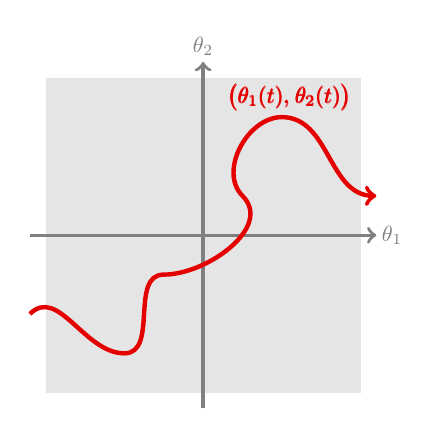
\begin{tikzpicture}
	\fill[black!10] (2,2) -- (-2,2) -- (-2, -2) -- (2, -2) -- cycle;
	\draw[black!50, very thick, ->] (-2.2,0) -- (2.2,0);
	\draw[black!50, very thick, ->] (0,-2.2) -- (0,2.2);
	\draw[red!90!black!100, ultra thick, ->] (-2.2,-1) to [out=45, in=180] (-1,-1.5) to [out=0, in=180] (-.5,-.5) to [out=0, in=-45] (.5,.5) to [out=135, in=180] (1, 1.5) to [out=0, in=180] (2.2,.5);
	\node[black!50] at (2.4, 0) {\scalebox{.8}{$\theta_1$}};
	\node[black!50] at (0, 2.4) {\scalebox{.8}{$\theta_2$}};	
	\node[red!90!black!100] at (1.1, 1.75) {\scalebox{.8}{$\pmb{\big(\theta_1(t),\ \!\theta_2(t)\big)}$}};
	\end{tikzpicture}
	$$
	\caption{General FM-synthesis from curves in the real plane.}
	\label{figure: ring modulation 2 dimensions}
	\end{figure}

%This begins to move into the realm of harmony. We pause our development of harmony here, and pick it back up in {\color{red} \S[...]}

\begin{example}
\normalfont
{\bf Ring modulation as a special case.}
Let us briefly remark here that, although it is not usually presented in this way, {\em ring modulation} in signal processing arises when we evaluate the real and imaginary parts of the monomial $xy$ at $x=e^{z_1}$ and $y=e^{z_2}$. In this way, ring modulation becomes a special case of the above discussion.
\end{example}

\begin{example}
\normalfont
{\bf Logarithmic representations.}
Consider the case of a single complex-valued function $z(t)=i2\pi\lambda t$ of the real variable $t$. How might we transform such a function. One obvious way is to consider all {\em $\RR$-affine transformations} of $t$, that is, all transformations that can be described by an $\RR$-linear polynomial:
	$$
	t
	\ \longmapsto\ 
	a+bt.
	$$
The group of all such transformations is denoted $\text{Aff}(\RR)$. It admits a normal decomposition
	$$
	0
	\longrightarrow
	\RR
	\longrightarrow
	\text{Aff}(\RR)
	\longrightarrow
	\RR^\times
	\longrightarrow
	1
	$$
that gives this group a semidirect product decomposition
	$$
	\text{Aff}(\RR)\ \cong\ \RR\rtimes\RR^\times.
	$$
We can effectively ``mod out'' the {\em translation} action by the normal subgroup $\RR\lhd\text{Aff}(\RR)$ by focus on the action of the non-normal, multiplicative subgroup $\RR^{\times}\subset\text{Aff}(\RR)$.

If we work with $e^{z}=e^{i2\pi\lambda t}$, the translation action $t\mapsto a+t$ by the normal subgroup $\mathbb{R}\rtimes\text{Aff}(\RR)$ amounts to phase shifting, as it takes
	$$
	e^{i2\pi\lambda t}
	\ \longmapsto\ 
	e^{i(2\pi\lambda t+\phi)},
	\ \ \ \text{where}\ 
	\phi=2\pi\lambda a.
	$$
If we take a musical perspective that ignores the effects of phase shifting, then we can focus on the action of the non-normal multiplicative subgroup $\RR^\times\subset\text{Aff}(\RR)$. It is common to use logarithmic coordinates for this group by writing $b=e^{s}$. We obtain transformations of the form
	$$
	e^{i2\pi\lambda t}
	\ \longmapsto\ 
	e^{i2\pi\lambda e^s t}.
	$$
Writing $\lambda=e^{s_0}$, this becomes
	$$
	e^{i2\pi e^{s_0} t}
	\ \longmapsto\ 
	e^{i2\pi e^{s_0+s} t}.
	$$
The charged particle dynamics in {\em Voice Leader\ \textemdash\ DISPL.} take place in something like the Lie algebra of the multiplicative group $\RR^\times$ that acts on the frequency specturm. Ignoring the negative component of this Lie algebra amounts to the assertion that we do not consider backward movement through time in musical contexts.

This leads us to the following questions for the case of $2$ independent variables $z_1$ and $z_2$.
\end{example}

\begin{question}
\normalfont
What is the right ``space'' to do dynamics in when there are two variables?... (frequency or log-frequency). 

There are going to be competing pictures, throughout these notes, for what level ``space'' should be taken at...
\end{question}

\begin{question}
\normalfont
What is the Lie bracket on the tangent space $T_{(\bold{q},\bold{p})}M$ of phase space $M$ at a state $(\bold{q},\bold{p})$?

\vskip .2cm

{\em Answer.} {\color{red} [Poisson algebra structure on the space of functions. The Lie algebra structure on the tangent space itself is known as the symplectic Lie algebra or the Lie algebra of Hamiltonian vector fields...]}

\vskip .2cm

{\em Relevance of the question to representations of algebraic groups.} {\color{red}\bf [...]}
\end{question}

\end{subsection}

\vskip .2cm

\begin{subsection}{Ring modulation versus products in representation theory}
	In representation theory, products arise from tensor constructions like tensor powers $V^{\otimes n}$, symmetric powers $\text{Sym}^{n}V$, and exterior powers $\Lambda^{n}V$ of representations $V$. The basic example of an element in one of these representations is the symmetric product $xy$ of two complex variables $x$ and $y$. If we're thinking in terms of irreducible representations, then it is natural to take 
	\begin{equation}\label{equation: variable assignment for product}
	x\ =\ e^{i2\pi\lambda t}
	\ \ \ \ \ \ \ \ \ \text{and}\ \ \ \ \ \ \ \ \ 
	y=e^{i2\pi\mu t}.
	\end{equation}
In this case, we have
	$$
	xy\ =\ e^{i2\pi(\lambda+\mu)\ \!t}.
	$$
Notice that here, products correspond to addition of frequencies.

	Ring modulation, on the other hand, corresponds to the product
	$$
	\text{Re}(x)\cdot\text{Re}(y).
	$$
If we let $x$ and $y$ take the values in Equation \ref{equation: variable assignment for product}, then this ring modulation product
	$$
	\text{sin}(2\pi\lambda t)\cdot\text{sin}(2\pi\mu t).
	$$
[...]
	\begin{equation}\label{equation: first expansion}
	\begin{array}{rcl}
	e^{i2\pi(\lambda+\mu)\ \!t}
	& \!\!=\!\!
	& \text{cos}\big(2\pi(\lambda+\mu)\ \!t\big)+i\ \text{sin}\big(2\pi(\lambda+\mu)\ \!t\big)
	\end{array}
	\end{equation}
[...]
	\begin{equation}\label{equation: second expansion}
	\begin{array}{rcl}
	e^{i2\pi\lambda t}\cdot e^{i2\pi\mu t}
	& \!\!=\!\!
	& \big(\text{cos}(2\pi\lambda t)+i\ \text{sin}(2\pi\lambda t)\big)
	\cdot
	\big(\text{cos}(2\pi\mu t)+i\ \text{sin}(2\pi\mu t)\big)
	\\[6pt]
	& \!\!=\!\!
	& \ \ \ \ \ \ \ \!\big(
	\text{cos}(2\pi\lambda t)\ \!\text{cos}(2\pi\mu t)
	-
	\text{sin}(2\pi\lambda t)\ \!\text{sin}(2\pi\mu t)
	\big)
	\\[6pt]
	&
	& 
	+\ i\ 
	\big(\text{cos}(2\pi\lambda t)\text{sin}(2\pi\mu t)+\text{sin}(2\pi\lambda t)\text{cos}(2\pi\mu t)\big)
	\end{array}
	\end{equation}
Identifying Equations \eqref{equation: first expansion} and \eqref{equation: second expansion}, we have
	\begin{equation}\label{equation: fragment A}
	\text{sin}(2\pi\lambda t)\cdot\text{sin}(2\pi\mu t)
	\ =\ 
	\text{cos}(2\pi\lambda t)\ \!\text{cos}(2\pi\mu t)
	-
	\text{cos}\big(2\pi(\lambda+\mu)\ \!t\big).
	\end{equation}
[...]
	\begin{equation}\label{equation: third expansion}
	\begin{array}{rcl}
	e^{i2\pi(\lambda-\mu)\ \!t}
	& \!\!=\!\!
	& \text{cos}\big(2\pi(\lambda-\mu)\ \!t\big)+i\ \text{sin}\big(2\pi(\lambda-\mu)\ \!t\big)
	\end{array}
	\end{equation}
[...]	\begin{equation}\label{equation: fourth expansion}
	\begin{array}{rcl}
	e^{i2\pi\lambda t}\cdot e^{-i2\pi\mu t}
	& \!\!=\!\!
	& \big(\text{sin}(2\pi\lambda t)+i\ \text{cos}(2\pi\lambda t)\big)
	\cdot
	\big(-\text{sin}(2\pi\mu t)+i\ \text{cos}(2\pi\mu t)\big)
	\\[6pt]
	& \!\!=\!\!
	& \ \ \ \ \ \ \ \!\big(
	-\text{sin}(2\pi\lambda t)\ \!\text{sin}(2\pi\mu t)
	-
	\text{cos}(2\pi\lambda t)\ \!\text{cos}(2\pi\mu t)
	\big)
	\\[6pt]
	&
	& 
	+\ i\ 
	\big(\text{sin}(2\pi\lambda t)\text{cos}(2\pi\mu t)-\text{cos}(2\pi\lambda t)\text{sin}(2\pi\mu t)\big)
	\end{array}
	\end{equation}
Identifying Equations \eqref{equation: third expansion} and \eqref{equation: fourth expansion}, we have
	\begin{equation}\label{equation: fragment B}
	\text{cos}(2\pi\lambda t)\cdot\text{cos}(2\pi\mu t)
	\ =\ 
	-\text{sin}(2\pi\lambda t)\ \!\text{sin}(2\pi\mu t)
	-
	\text{cos}\big(2\pi(\lambda-\mu)\ \!t\big).
	\end{equation}
Putting Equations \eqref{equation: fragment A} and \eqref{equation: fragment B} together, we arrive at the identity
	$$
	2\ \text{sin}(2\pi\lambda t)\ \!\text{sin}(2\pi\mu t)
	\ =\ 
	\text{cos}\big(2\pi(\lambda+\mu)\ \!t\big)+\text{cos}\big(2\pi(\lambda-\mu)\ \!t\big),
	$$
more commonly written
	\begin{equation}\label{equation: trig identity}
	\text{sin}(2\pi\lambda t)\cdot\text{sin}(2\pi\mu t)
	\ =\ 
	\frac{1}{2}\text{cos}\big(2\pi(\lambda+\mu)\ \!t\big)+\frac{1}{2}\text{cos}\big(2\pi(\lambda-\mu)\ \!t\big)
	\end{equation}

	The point of all of this is that we have competing interpretations of signal multiplication coming from the inequality
	$$
	\text{Re}(xy)\ \neq\ \text{Re}(x)\cdot\text{Re}(y)
	$$
for complex variables $x$ and $y$.
	
\begin{question}
{\bf A purely Galois version of the identity in Equation \eqref{equation: trig identity}?}
\normalfont
We can re-interpret the factor $e^{-i2\pi\mu t}$ in Equation \eqref{equation: fourth expansion} as the Galois conjugate
	$$
	e^{-i2\pi\mu t}=\sigma(e^{i2\pi\mu t}),
	$$
where $\sigma$ denotes the unique non-trivial automorphism in $\text{Gal}(\CC/\RR)$. In this way, the identity in Equation \eqref{equation: trig identity} can be written in the non-trigonometric form
	\begin{equation}\label{equation: non-trig form}
	\text{Re}(x)\text{Re}(y)
	\ =\ 
	\frac{1}{2}\text{Re}(xy)+\frac{1}{2}\text{Re}\big(x\cdot\sigma(y)\big).
	\end{equation}
We can think of the $\RR$-linear map $\text{Re}:\CC\longrightarrow\RR$ as a projection operation with respect to the $\RR$-linear basis $\{1,i\}$ in $\CC$, where $i$ is a root of the irreducible quadratic polynomial $x^2+1\in\RR[x]$. If we let $\omega$ be the root of some other irreducible quadratic polynomial $x^2+ax+b\in\RR[x]$, we get a new $\RR$-linear basis $\{1,\omega\}$ for $\CC$, and thus a {\em new} projection
	$$
	\text{pr}_{\omega}:\CC\longrightarrow\RR.
	$$
Is it the case that this new projection satisfies the naive analogue of Equation \eqref{equation: non-trig form}, namely
	$$
	\text{pr}_{\omega}(x)\text{pr}_{\omega}(y)
	\ =\ 
	\frac{1}{2}\text{pr}_{\omega}(xy)+\frac{1}{2}\text{pr}_{\omega}\big(x\cdot\sigma(y)\big)?
	$$
My first guess is that this can't be correct, and that it requires some modification coming from the polynomial $x^2+ax+b$.

	A further generalization might be some formula for any ``norm-type'' product
	$$
	\prod_{j,g\in\text{enum}\big(\text{Gal}(E/F)\big)}
	\!\!\!\!\!\!\!\!\!\!\!g(x_{j}).
	$$
My initial guess would be something of the form
	$$
	\prod_{j,g\in\text{enum}\big(\text{Gal}(E/F)\big)}
	\!\!\!\!\!\!\!\!\!\!\!g(x_{j})
	\ \ \ =\ \ \ 
	\frac{1}{\#\text{Gal}(E/F)}
	\sum_{g\in\text{Gal}(E/F)}\!\!\!\!\!\big(?\big)
	$$
Probably the right place to look for the answer is some general ``norm-to-trace'' formula in class field theory.
\end{question}
	
\end{subsection}

\vskip .2cm

\begin{subsection}{Homogenous linear combinations of independent complex variables}
If $x$ and $y$ are independent complex variables, then a $\CC$-linear combination of monomials in $x$ and $y$, say
	\begin{equation}\label{homogeneous linear comb 1}
	a_{1}x^{m_1}y^{n_1}
	+
	a_{2}x^{m_2}y^{n_2}
	+
	\cdots
	+
	a_{\ell}x^{m_\ell}y^{n_\ell},
	\ \ \ a_1,a_2,\dots,a_\ell\in\CC
	\end{equation}
is {\em homogeneous of degree $d$} if $m_i+n_i=d$ for all $1\le i\le \ell$, in other words, if all monomials $x^my^n$ in the linear combination have the same {\em total degree} $m+n$, equal to $d$. When the linear combination in Equation \eqref{homogeneous linear comb 1} is homogeneous of degree $d$, we refer to it as a {\em homogeneous polynomial of degree $d$} in the variables $x$ and $y$ over $\CC$.

Notice that, from a musical perspective, a homogeneous linear combination in Equation \eqref{homogeneous linear comb 1} combines two distinct ideas in a way that isn't possible with a single variable. It packages multiple instances of ring modulation into a single chord-like structure. Indeed, 

The general homogeneous polynomial of degree $d$ in $x$ and $y$ can be written
	$$
	f(x,y)
	\ =\ 
	a_{0}x^d+a_1x^{d-1}y+a_2x^{d-2}y^2+\cdots+a_{d-1}xy^{d-1}+a_{d}y^d,
	$$
with coefficients $a_0,a_1,\dots,a_d\in\CC$. We can write this more succinctly as
	$$
	f(x,y)
	\ =\ 
	\sum_{n=0}^{d}a_nx^{d-n}y^n.
	$$
Evaluating this polynomial at $x=e^{z_1}$ and $y=e^{z_2}$, we obtain
	\begin{equation}\label{equation: homogeneous eval at e^z}
	f(e^{z_1},e^{z_2})
	\ =\ 
	\sum_{n=0}^{d}a_{n}A_{1}^{d-n}A_{2}^{n}e^{i2\pi\big(\tfrac{d-n}{P_1}\theta_1+\tfrac{n}{P_2}\theta_2\big)}.
	\end{equation}
To get a slightly clearer picture of this, let us assume that $a_i=1$ for all $0\le i\le d$ {\color{red} [change $i$ to different letter...]} and that $A_1=A_2=1$. Then the right-hand side of Equation \eqref{equation: homogeneous eval at e^z} becomes
	\begin{equation}\label{equation: all amplitudes =1}
	\sum_{n=0}^{d}e^{i2\pi\big(\tfrac{d-n}{P_1}\theta_1+\tfrac{n}{P_2}\theta_2\big)}.
	\end{equation}
We play with this expression a bit more in Example \ref{example: relationship to standard chords} below.

\begin{example}\label{example: relationship to standard chords}
\normalfont
{\color{red} [...]}

{\bf Special case: $\pmb{\theta_1=\theta_2}$ and $\pmb{P_1=P_2}$.}
{\color{red} [...]}
	Equation \eqref{equation: all amplitudes =1} becomes
	$$
	(d+1)e^{i2\pi\tfrac{d}{P}\theta}
	\ =\ 
	(d+1)e^{i2\pi d\lambda\theta}
	$$

{\bf Special case: $\pmb{\theta_1=0}$.}
{\color{red} [...]}
	Equation \eqref{equation: all amplitudes =1} becomes
	$$
	\sum_{n=0}^{d}e^{i2\pi\tfrac{n}{P}\theta}
	\ =\ 
	1
	+
	e^{i2\pi\tfrac{1}{P}\theta}
	+
	e^{i2\pi\tfrac{2}{P}\theta}
	+
	\dots
	+
	e^{i2\pi\tfrac{d}{P}\theta},
	$$
or in terms of frequency,
	$$
	f(1,e^{i2\pi\lambda\theta})
	\ =\ 
	1
	+
	e^{i2\pi \lambda\theta}
	+
	e^{i2\pi 2\lambda\theta}
	+
	\dots
	+
	e^{i2\pi d \lambda\theta}.
	$$
Ignoring the constant term ``$1$,'' this is just an equi-voiced\footnote{\ We say that a chord is {\em equi-voiced} if the notes of a chord are equally loud. I don't know if this is standard terminology.} overtone chord with root at $\lambda\ \text{Hz}$, and including overtones $1$ through $d$.

If we let $A_1=1$ and $A_2=\varepsilon$, where $0<\varepsilon <1$, then this becomes
	$$
	f(1,\varepsilon e^{i2\pi\lambda\theta})
	\ =\ 
	1
	+
	\varepsilon e^{i2\pi \lambda\theta}
	+
	\varepsilon^2 e^{i2\pi 2\lambda\theta}
	+
	\dots
	+
	\varepsilon^d e^{i2\pi d \lambda\theta}.
	$$
This is the same overtone chord, but with voicing that falls of like a geometric series as we move up the overtone scale.
\end{example}

\begin{question}
\normalfont
{\color{red} [Voicing and orchestration questions...]}
\end{question}


\begin{remark}
\normalfont
{\color{red} [Model movement of several $(\theta_1,\ \theta_2)$-pairs on particle dynamics in $2$-dimensional space. This provides an FM version of the particle dynamics experiment from {\em Voice Leader\ \textemdash\ DISPL.}...]}
\end{remark}
[...]
\end{subsection}

\begin{subsection}{A gestural notation.}
\ 
{\color{red} [...]}

\end{subsection}

\end{section}

\vskip 1cm

\begin{section}{Representations of the special linear group $\text{SL}_{2}(\CC)$.}

\begin{subsection}{Sources}
	\begin{enumerate}[{\bf\ \ \ \ \ \ 1.}]
	\item
	\cite{FH}
	\item
	\cite{Proc}
	\item
	\cite{Knapp86}
	\item
	\cite{Knapp02}
	\end{enumerate}
\end{subsection}

\begin{subsection}{The Cartan-Weyl basis.} The $3$-dimensional Lie algebra
	$$
	\mathfrak{sl}_2(\CC)
	\ =\ 
	\left\{
	\left(\!\begin{array}{cc}a & b \\ c & \!\!-a\end{array}\!\right)\in\text{Mat}_{2\times2}(\CC)
	\right\}
	$$
admits a standard basis, sometimes called the {\em Cartan-Weyl basis}, given by
	$$
	E:=\left(\!\begin{array}{cc}0 & 1 \\ 0 & 0\end{array}\!\right),
	\ \ \ \ \ \ 
	H:=\left(\!\begin{array}{cc}1 & 0 \\ 0 & \!\!-1\end{array}\!\right),
	\ \ \ \ \ \ 
	\text{and}
	\ \ \ \ \ \ 
	F:=\left(\!\begin{array}{cc} 0 & 0 \\ 1 & 0\end{array}\!\right).
	$$
The $1$-parameter subgroups gotten by exponentiation of these basis vectors have general element
	$$
	e^{zE}
	\ =\ 
	\text{I}+zE+\frac{z^2}{2}{\color{red} \cancelto{0}{{\color{black} E^2}}}+\frac{z^3}{3!}{\color{red} \cancelto{0}{{\color{black} E^3}}}+\cdots
	\ =\ 
	\left(\!\begin{array}{cc} 1 & z \\ 0 & 1\end{array}\!\right),
	$$
	$$
	e^{zF}
	\ =\ 
	\text{I}+zF+\frac{z^2}{2}{\color{red} \cancelto{0}{{\color{black} F^2}}}+\frac{z^3}{3!}{\color{red} \cancelto{0}{{\color{black} F^3}}}+\cdots
	\ =\ 
	\left(\!\begin{array}{cc} 1 & 0 \\ z & 1\end{array}\!\right),
	$$
and
	$$
	\begin{array}{rclcl}
	e^{zH}
	& \!\!=\!\! &
	I+zH+\frac{z^2}{2}H^2+\frac{z^3}{3!}H^3+\cdots
	\\[20pt]
	& \!\!=\!\! &
	\left(\ \!\begin{array}{cc} 1+z+\tfrac{z^2}{2}+\tfrac{z^3}{3!}+\cdots & 0 \\[7pt] 0 & 1-z+\tfrac{z^2}{2}-\tfrac{z^3}{3!}+\cdots\end{array}\!\ \right)
	& \!\!=\!\! &
	\left(\!\begin{array}{cc} e^z & 0 \\ 0 & e^{-z}\end{array}\!\right),
	\end{array}
	$$
respectively. One recurring theme in these notes is the question ``should we work in the space where our variable is $z$, or in the space where are variable is $q=e^{z}$. Note, though, that this distinction gets confused in $\text{SL}_{2}(\CC)$, since the complex parameter $z$ acts by multiplication directly in the $1$-parameter subgroups $$\{e^{zE}:z\in\CC\}\ \ \text{and}\ \ \{e^{zF}:z\in\CC\}\subset\text{SL}_{2}(\CC),$$ but acts through multiplication by in the $1$-parameter subgroup $$\{e^{zH}:z\in\CC\}\subset\text{SL}_{2}(\CC).$$

Every element $\left(\begin{smallmatrix} a & b \\ c & d\end{smallmatrix}\right)\in\text{SL}_{2}(\CC)$ admits a factorization
	$$
	\left(\!\begin{array}{cc}a & b \\ c & d\end{array}\!\right)
	\ =\ 
	e^{u E}e^{v H}e^{w F}
	\ =\ 
	\left(\!\begin{array}{cc}1 & w \\ 0 & 1\end{array}\!\right)
	\left(\!\begin{array}{cc}e^{v} & 0 \\ 0 & e^{-v}\end{array}\!\right)
	\left(\!\begin{array}{cc}1 & 0 \\ u & 1\end{array}\!\right)
	$$
for some $u,v,w\in\CC$ {\color{red} [Not true. A certain conjugation is needed to get matrices $\left(\begin{smallmatrix} 0 & b \\ \!\!-\tfrac{1}{b} & 0\end{smallmatrix}\right)$... What is the correct statement here. Some kind of decomposition theorem for the Lie group?...Bruhat decomposition?...]}. To compute $u,v,w$, observe that the matrix product on the right is equal to
	$$
%	\left(\!\begin{array}{cc}1 & w \\ 0 & 1\end{array}\!\right)
%	\left(\!\begin{array}{cc}e^v & 0 \\ ue^{-v} & e^{-v}\end{array}\!\right)
%	\ =\ 
	\left(\!\begin{array}{cc}e^v+uwe^{-v} & we^{-v} \\ ue^{-v} & e^{-v}\end{array}\!\right),
	$$
hence
	$$
	d=e^{-v},
	\ \ \ \ \ \ 
	w=b/d,
	\ \ \ \ \ \ 
	u=c/d
	$$
{\color{red} [...confusing myself... need to come back to this...]} The thing that's confusing me is how $\left(\begin{smallmatrix} 0 & b \\ \!\!-\tfrac{1}{b} & 0\end{smallmatrix}\right)$ appears. Maybe the 1-parameter subgroups at the identity $I=\left(\begin{smallmatrix} 1 & 0 \\ 0 & 1\end{smallmatrix}\right)\in\text{SL}_{2}(\CC)$ doesn't reach any of the cell
	\begin{equation}\label{stratum 1}
	S:=\left\{\left(\begin{smallmatrix} 0 & b \\ \!\!-\tfrac{1}{b} & 0\end{smallmatrix}\right):b\in\CC^\times\right\}
	\ \subset\ 
	\text{SL}_{2}(\CC).
	\end{equation}
What is the product of two elements of this cell like?
	$$
	\left(\begin{matrix} 0 & b \\ \!\!-\tfrac{1}{b} & 0\end{matrix}\right)
	\left(\begin{matrix} 0 & -\tfrac{1}{c} \\ c & 0\!\!\end{matrix}\right)
	\ =\ \left(\begin{matrix} bc & 0 \\ 0 & \tfrac{1}{bc}\end{matrix}\right)
	\ \in\ \{e^{zH}:z\in\CC\}.
	$$
In other words, the square of the stratum defined in Equation \eqref{stratum 1} is the $1$-parameter subgroup generated by the exponentiation of the basis field $H\in\mathfrak{sl}_{2}(\CC)$.



{\color{red} [Factorizations coming from other permutations of these $3$ factors...]}

{\color{red} [...]}
\end{subsection}

\begin{subsection}{Action of $\text{SL}_{2}(\CC)$ on $\CC[x,y]$}
We let $\text{SL}_{2}(\CC)$ act on $\CC[x,y]$ through its inverse action on the argument $(x,y)$ of each function $f(x,y)\in\CC[x,y]$. Thus the matrix $\left(\begin{smallmatrix}a & b\\ c & d\end{smallmatrix}\right)\in\text{SL}_{2}(\CC)$ acts on each $f(x,y)\in\CC[x,y]$ via the action of its inverse $\left(\begin{smallmatrix}d & -b\ \\ -c\  & a\end{smallmatrix}\right)$
\end{subsection}

\begin{subsection}{Irreducible representations of $\text{SL}_2(\CC)$ in $\CC[x,y]$}
[...]
\end{subsection}

\begin{subsection}{The irreducible $2$-dimensional representation of $\text{SL}_2(\CC)$}
[...]
\end{subsection}

\begin{subsection}{The irreducible $3$-dimensional representation of $\text{SL}_2(\CC)$}
[...]
\end{subsection}

\begin{subsection}{``Harmonic movement'' for $\text{SL}_2(\CC)$}

\begin{question}\label{question: what is harmonic movement}
\normalfont
What sort of movement through the category $\bold{Rep}\big(\text{SL}_{2}(\CC)\big)$ is the ``correct'' generalization of the movement through $\bold{Rep}\big(\mathbb{S}^{1}\big)$ that corresponds to $\ZZ$-multiplicative movement through the terms of a Fourier series?

\vskip .3cm

\noindent
{\em Temporary answers.} There are many reasonable candidates:
	\begin{enumerate}[{\em\ \ \ \ \ \ {Answer \ref{question: what is harmonic movement}.}1.}]
	\item
	Inductive/restrictive functorial movement along homomorphisms $G\longrightarrow\text{SL}_{2}(\CC)$ and/or $\text{SL}_{2}(\CC)\longrightarrow G$;
	\item
	Movement along functors $\text{Hom}(V_{n},-)$;
	\item
	Movement along functors $T^{n}=(-)^{\otimes n}$;
	\item
	Movement along functors $\text{Sym}^{n}$;
	\item
	Movement along functors $\Lambda^{n}$.
	\end{enumerate}
{\color{red} [Explain issue of plethysm/fusion rules...]}
\end{question}

[...]
\end{subsection}

\begin{subsection}{Plethysm}
[...]
\end{subsection}

\begin{subsection}{A gestural notation.}
\ 
{\color{red} [...]}

\end{subsection}

\end{section}

\vskip 1cm

\begin{section}{Hamiltonian optics and representations of the symplectic group $\text{Sp}_{2n}(\CC)$}

\begin{subsection}{Sources}
	\begin{enumerate}[{\bf\ \ \ \ \ \ 1.}]
	\item
	\cite{GS}
	\end{enumerate}
\end{subsection}
[...]
\end{section}

\vskip 1cm

\begin{section}{Homogeneous spaces}

\begin{subsection}{Sources}
	\begin{enumerate}[{\bf\ \ \ \ \ \ 1.}]
	\item
	\cite{Serre}
	\item
	\cite{Tim}
	\item
	\cite{Schmitt}
	\end{enumerate}
\end{subsection}

\end{section}

%$$
%10,668,000
%\ =\ 
%\left(\!\!
%\begin{array}{c}
%128\\
%4
%\end{array}
%\!\!\right)
%$$
%
%$$
%\mathbb{E}[f]
%\ =\ 
%\int_{S}f(s)ds
%$$
%
%$$
%\underset{
%{\smaller\smaller\smaller\smaller\smaller
%\begin{array}{c}
%\text{paths $\gamma$ in $S$}
%\\
%\text{starting at $s$}
%\end{array}
%}
%}{\text{argmax}}
%\ G(\gamma)
%$$
%
%$$
%\mathbb{E}_\pi[G|s]
%\ =\ 
%\int_{\!\!\mathscr{P}\!(S,s)}\!\!\!\!G(\gamma)\ d\pi
%$$
%
%$$
%\mathbb{E}_{\pi}[G|s]
%\ =\!\!
%\underset{
%{\smaller\smaller\smaller\smaller
%\begin{array}{c}
%\text{actions}
%\\
%\alpha\ \text{at}\ s
%\end{array}
%}
%}{\sum}
%\!\!\!\!
%\Big(
%\Delta_{\alpha}G
%+
%\mathbb{E}\big[G\big|\alpha(s)\big]
%\Big)
%\ 
%p_{\pi}(\alpha|s)
%$$
%
%$$
%\mathbb{E}_{\pi}[G|\alpha,s]
%\ =\ 
%\Delta_{\alpha}G
%+
%\mathbb{E}\big[G\big|\alpha(s)\big]
%$$
%
%$$
%\mathbb{E}_{\pi}[G|\alpha,s]
%\ =\ 
%\Delta_{\alpha}G
%\ +\!\!\!\!\!\!
%\underset{
%{\smaller\smaller\smaller\smaller
%\begin{array}{c}
%\text{actions}
%\\
%\beta\ \text{at}\ \alpha(s)
%\end{array}
%}
%}{\sum}
%\!\!\!\!
%\mathbb{E}\big[G\big|\beta,\alpha(s)\big]
%\cdot
%p_{\pi\!}\big(\beta\big|\alpha(s)\big)
%$$
%
%$$
%\mathbb{E}_{\pi}[G|\alpha,s]
%\ =\ 
%\Delta_{\alpha}G
%\ +\ 
%\mathbb{E}\big[G\big|\beta_{\text{{\smaller\smaller\smaller\smaller\smaller best}}},\alpha(s)\big]
%$$
%
%$$
%\mathbb{E}[G|\alpha_i,s_i]
%\ =\ 
%R_{\alpha_i}+R_{\alpha_{i+1}}+R_{\alpha_{i+2}}+\cdots+R_{\alpha_n}
%$$








\vskip .75cm

\bibliographystyle{alpha}
\bibliography{SL_2C}

\end{document}
